%===============================================================================
% ifacconf.tex 2025-07-31 jpuente  
% 2022-11-11 jpuente change length of abstract
% 2025-07-31 jldiez added section on the use of AI
% Template for IFAC meeting papers
% Copyright (c) 2025 International Federation of Automatic Control
%===============================================================================
\documentclass{ifacconf}

\usepackage{graphicx}      % include this line if your document contains figures
\usepackage{natbib}        % required for bibliography
\graphicspath{{../}{../img/}{img/}}

%===============================================================================

\usepackage{algorithmic}

\usepackage{textcomp}

% \usepackage{comment}

%\usepackage{graphicx}      % include this line if your document contains figures
%\usepackage{natbib}        % required for bibliography
%===============================================================================
% Needed to meet printer requirements.
 \usepackage{latexsym,amssymb,amsfonts}
\usepackage[applemac]{inputenc}
\usepackage{rotating}
%\usepackage{graphicx}
\usepackage{epstopdf}
% \usepackage{subfigure}
%\usepackage{color}
%\usepackage{xcolor}
%
%\usepackage{color}
\usepackage[dvipsnames]{xcolor}
%
\usepackage[normalem]{ulem}
% \usepackage{isolatin1}
%\usepackage{caption}
\usepackage{subcaption} 
\usepackage{booktabs}

%\usepackage{array,multirow,makecell}
%\usepackage{placeins}
%\usepackage{stackengine}
%\usepackage{hyperref}
\usepackage{fancybox}
\usepackage{colortbl}
\usepackage{float}
\usepackage{comment}
\usepackage{mathdots}
%\usepackage{lmodern}
%%%%%%%%%%%%%%%%%%%%%%%%%%%%%%%%%%%%%%%%%%%%%%%%%%%%%%%%%
\usepackage{dblfloatfix}    % To enable figures at the bottom of page
\usepackage{placeins}
\usepackage{marginnote}
\usepackage{url}
% \usepackage{hyperref}
%\usepackage{empheq}
\usepackage[overload]{empheq}

\usepackage{bm}

%%%%%%%%%%%%%%%%%%%%%%%%%%%%%%%%%%%%%%%%%%%%%%%%%%%%%%%%%
\usepackage{tikz}
\usetikzlibrary{circuits.ee.IEC}
\usepackage[european resistor, european voltage, european current]{circuitikz}
\usetikzlibrary{arrows, shapes, positioning}
\usetikzlibrary{decorations.markings, decorations.pathmorphing,
decorations.pathreplacing}
\usetikzlibrary{calc,patterns,shapes.geometric}
\usetikzlibrary{shapes.multipart, positioning, patterns, backgrounds}
\tikzstyle{titlebox}=[rectangle,inner sep=10pt,inner ysep=10pt,draw]%
\usetikzlibrary{arrows.meta}
\usetikzlibrary{matrix, fit}

%%%%%%%%%%%%%%%%%%%%%%%%%%%%%%%%%%%%%%%%%%%%%%%%%%%%%%%%%%%%%

\def\blacksquare{\hbox{\vrule width 4pt height 4pt depth 0pt}}
\def\square{\hbox{\vrule\barox{\hrule\phantom{o}\hrule}\vrule}}
\def\qed{\hfill \square}
\def\qedp{\rightline{$\blacksquare$}}
\def\EXPT{\mathop{{\rm E}}}
\def\MIN{\mathop{{\rm min}}}
\def\MAX{\mathop{{\rm max}}}
\def\LIM{\mathop{{\longrightarrow}}}
\def\UNION{\mathop{\bigcup}}
\def\INTERSECT{\mathop{\bigcap}}
\def\ARGMIN{\mathop{{\rm argmin}}}
\def\ARGMAX{\mathop{{\rm argmax}}}
\def\TOUND{\mathop{\longrightarrow}}
\def\col#1{\mathop{{\rm col}\,\left(\,#1\,\right)}}
\def\eqref#1{(\ref{#1})}
\newcommand{\widebox}[2][0.5em]{\fbox{\hspace{#1}$\displaystyle #2$\hspace{#1}}}



\def\rank{\mathop{{\rm rank}}}

% User definition from Shengya
\def\V{\mathcal{V}} % the set of vehicle
\def\E{\mathcal{E}} % the set of edge
\def\G{\mathcal{G}} % graph
\def\A{\mathcal{A}} % adjacency matrix 
\def\W{\mathcal{W}} % weighted adjacency matrix
\def\L{\mathcal{L}} % Laplacian matrix
\def\N{\mathcal{N}} % neighbors
\def\LO{\mathcal{LO}} % the set of observer
\def\DO{\mathcal{DO}} % the set of observer
\def\diag#1{\mathop{{\rm diag}\,\left(\,#1\,\right)}}
\def\ST{\mathcal{ST}} % Self trust
\def\LT{\mathcal{LT}} % Local trust
\def\DT{\mathcal{DT}} % Distributed trust 
\def\VT{\mathcal{VT}} % Vehicle trust 
\def\AT{\mathcal{AT}} % Aggregation trust
\def\T{\mathcal{T}} % Aggregation trust
\def\O{\mathcal{O}} % opinion
\def\nn{\mathrm{NN}}
\def\uio{\mathrm{UIO}}
\def\refx{\mathrm{ref}}
\def\Lo{L}


% User Defined Color based on RGB
\definecolor{userblue}{RGB}{31,119,180}
\definecolor{userorange}{RGB}{255,127,14}
\definecolor{usergreen}{RGB}{44,160,44}
\definecolor{userpurple}{RGB}{148,103,189}

\definecolor{blue1}{RGB}{31,119,180}    % 车辆/物理层
\definecolor{orange1}{RGB}{255,127,14}  % 本地观测器
\definecolor{green1}{RGB}{44,160,44}    % 信息层/通信
\definecolor{purple1}{RGB}{148,103,189} % 分布式观测器
\definecolor{rose1}{RGB}{227, 119, 194}

%%%
%\newtheorem{prb}{\it Problem}%[section]
%\newtheorem{theorem}{\it Theorem}%[section]
%\newtheorem{lemma}{\it Lemma}%[section]
%\newtheorem{definition}{\it Definition}
%\newtheorem{remark}{\it Remark}%[section]
%\newtheorem{assumption}{\it Assumption}%[section]
%\newtheorem{example}{\it Example}%[section]b
%\newtheorem{annex}{\it Annex}%[section]b
% \newtheorem{prop}{\it Proposition}%[section]b

\newtheorem{prb}{\it Problem}%[section]
\newtheorem{theorem}{\it \textbf{Theorem}}%[section]
\newtheorem{proposition}{\it \textbf{Proposition}}%[section]
\newtheorem{lemma}{\it \textbf{Lemma}}%[section]
\newtheorem{definition}{\it \textbf{Definition}}
\newtheorem{remark}{\it \textbf{Remark}}%[section]
\newtheorem{assumption}{\it \textbf{Assumption}}%[section]
\newtheorem{example}{\it \textbf{Example}}%[section]b
\newtheorem{annex}{\it \textbf{Annex}}%[section]b


\newtheorem{alert}{\color{red}\it Alert Remark}
% \newtheorem{pf}{\it Proof}%[section]b




\def\BibTeX{{\rm B\kern-.05em{\sc i\kern-.025em b}\kern-.08em
    T\kern-.1667em\lower.7ex\hbox{E}\kern-.125emX}}

\tikzset{global scale/.style={
    scale=#1,
    every node/.append style={scale=#1}
  }
}

\usepackage{arydshln} % permet d'avoir des lignes pointillées
\usepackage{dashrule}

%===============================================================================
\begin{document}
\begin{frontmatter}

\title{Learning with Unknown Input Observers for Robust Nonlinear Estimation}  
% Title, preferably not more than 10 words.
% Title, preferably not more than 10 words.

\thanks[footnoteinfo]{This work was supported by SEGULA Engineering.}

\author[First]{Q.H. Nguyen} 
\author[First]{L. Qi}
\author[First]{A. Zemouche}
\author[First]{H. Rafaralahy}
\author[Second]{M. Haddad}

\address[First]{Universit\'e de Lorraine, CNRS, CRAN, F-57000 Metz (e-mail: quang-huy.nguyen@univ-lorraine.fr).}
\address[Second]{SEGULA Engineering, 19 rue d'Arras, 92000 Nanterre, France (e-mail: madjid.haddad@segula.fr)}
% \address[Third]{Electrical Engineering Department, 
   % Seoul National University, Seoul, Korea, (e-mail: author@snu.ac.kr)}

\begin{abstract}                % Abstract of 50--100 words
This paper proposes a hybrid estimator for vehicle systems with unmodeled dynamics. A generalized unknown input observer provides bounded physics-based estimates when classical rank conditions are relaxed through output derivatives. These estimates supervise a neural adaptive observer that learns a state-dependent approximation of the unknown input. LMI conditions certify $\mathcal{H}^{1}$ and $\mathcal{L}_{2}$ estimation bounds, and vehicle simulations show improved trajectory tracking and tire-force residual reconstruction.
\end{abstract}

\begin{keyword}
Robust estimation, model learning, neural networks.
\end{keyword}

\end{frontmatter}




\section{Introduction}\label{sec_introduction}
%%% NEWWSSS Introduction 

State estimation is central to autonomous vehicle control, where safety depends on accurate knowledge of states and disturbances. Traditional methods rely on physics-based models \citep{State_Esti2017}, but tire-road friction, aerodynamic effects, and parameter variations are difficult to model and can degrade estimation performance.

Neural networks (NNs) can approximate such nonlinearities \citep{2006Apdat,HO_GP}. However, pure online learning may behave unpredictably under data shifts and lacks the guarantees required in safety-critical systems. This motivates hybrid observer-learning architectures.

A major limitation of existing hybrid observers is the standard matching/rank condition~\citep{Trinh:TAC08,chaouche2022unknown}. For practical vehicle sensor sets, this condition may fail, preventing exact unknown-input decoupling. Existing workarounds often amplify noise, increase sensing cost, or impose restrictive disturbance assumptions.

To overcome these limitations, this paper proposes a teacher--student estimation architecture. A generalized UIO provides bounded physics-based unknown-input estimates, while a neural adaptive observer learns a state-dependent approximation of the unknown dynamics. The contributions are a rank-relaxed UIO using output derivatives, a UIO-supervised neural learning framework, and LMI-based stability conditions.



% %%%% OLDs introduction

%     State estimation is crucial for controlling and monitoring complex systems across various disciplines. Traditional methods often rely on carefully crafted, physics-based models \cite{State_Esti2017}. However, these models frequently struggle to capture the intricate nonlinearities inherent in real-world systems, leading to inaccurate state estimates that can compromise both optimal performance and safety.


% In recent years, machine learning, particularly neural networks (NNs), has emerged as a powerful tool for addressing the limitations of traditional methods. Neural networks have been extensively investigated for system identification, state observation, and control of nonlinear systems, both in offline and online environments \cite{2006Apdat, HO_GP}. Their adaptive behavior and ability to approximate complex, nonlinear functions make them well-suited for state estimation tasks, even in the absence of prior knowledge about system dynamics. However, neural networks face challenges in online learning scenarios, where small changes in input data can lead to disproportionately large outputs, compromising reliability and stability.

% Recent advancements have sought to address these challenges by combining data-driven learning with traditional observer design techniques. For instance, some works employ neural networks with smooth, continuous-time weight update laws or basis expansions to model system dynamics, integrating these models into observers with linear output injection terms \cite{Jeon_Neraul_LMI}. While these approaches have demonstrated promise, they often require solving large sets of linear matrix inequalities to ensure joint convergence, resulting in complex neural network models and a high number of tunable parameters. These limitations hinder the practical applicability of such frameworks.

% % In this work, we propose an approach to state estimation that leverages the strengths of both physics-based modeling and data-driven learning. While UIO observers offer robustness and simplicity, they often struggle with capturing fast-changing nonlinearities. In contrast, neural networks excel at modeling complex, time-varying dynamics, but may lack robustness, especially in safety-critical applications. Therefore, we combine both approaches to achieve an estimator that is both adaptive and stable, effectively handling unmodeled dynamics and external disturbances.

% Specifically, our method integrates two observers: a General UIO observer and a Neural Adaptive Observer. The UIO observer exploits prior knowledge of the system model to provide an initial estimate of the unknown dynamics, while the neural observer refines this estimate by incorporating reference errors and adapting to unmodeled behaviors. This layered architecture ensures that both the state estimation error and the uncertain dynamics estimation error are bounded. By embedding this structure into the loss function, we achieve reliable model learning during online deployment. This is particularly advantageous in systems subject to persistent uncertainties that are difficult to model explicitly, such as variable road friction or aerodynamic drag.

% To further enhance adaptability, we introduce a continuous learning framework that maintains estimator performance in the presence of long-term, unpredictable disturbances. Unlike existing methods that treat disturbances separately using tools such as disturbance observers or unknown input observers \cite{khalil2020fault, PIO_2015}, our approach unifies the treatment of unknown dynamics and disturbances in a single neural learning loop. Leveraging a cascading neural network architecture \cite{KNOD_sate_esti}, our method retains past knowledge while learning new patterns online. A key component is a forgetting mechanism, which allows the neural network to prioritize recent dynamics without discarding useful historical information, thereby improving long-term estimation accuracy.

% % After the learning algorithm has converged, we propose an additional step to further enhance the observer's performance. This involves redesigning the observer based on the information captured by the learned Neural ODE model, optimizing the system's ability to estimate states accurately.

% % By combining neural network learning with prior model knowledge and robust learning guarantees, this work represents a significant advancement in state estimation. The proposed approach is highly relevant for applications that require precise state knowledge, such as robotics and chemical process control. Our method ensures safe learning during training and leverages the learned model to deliver superior observer performance in real-world environments.

% %{\color{red}
% %The remainder of this paper is organized as follows. Section~\ref{sec2} presents the problem formulation. Section~\ref{sec3} introduces the neural adaptive observer used in this work. Sections~\ref{sec4} and~\ref{sec5} detail the estimation of the unknown nonlinear function of the system using neural networks. Finally, Section~\ref{sec6} provides simulation results obtained by applying the proposed estimation techniques to a vehicle trajectory tracking scenario.
% %}



% % $$
% %  \textcolor{red}{***\text{ BEGIN ALI ***}}
% % $$


% %%%% OLDs introduction

%=====================================


\section{Problem Formulation and Motivation}\label{sec2}
%
In this paper, we consider the class of continuous-time nonlinear systems in state-space form described by the following equations:

\begin{equation}\label{sys_1}
    \begin{array}{l}
        \dot{x} = \varphi(x,u) + B\mu_{x}  \\
        y = Cx, 
    \end{array}
\end{equation}
where $x\in \mathcal{X} \subseteq\mathbb{R}^{n_x}$ is the state vector, $y\in\mathbb{R}^{n_y}$ is the output measurement, $u\in\mathcal{U} \subseteq\mathbb{R}^{n_u}$ is the control input, and $\mu_{x}\in\mathbb{R}^{n_{\mu}}$ is an unknown input signal that represents unmodeled dynamics and external disturbances. The matrices $C\in\mathbb{R}^{n_y}\times\mathbb{R}^{n_x}$ and $B\in\mathbb{R}^{n_x}\times\mathbb{R}^{n_{\mu}}$ are constant and known matrices. The function $\varphi: \mathcal{X} \times \mathcal{U} \to \mathbb{R}^{n_x}$ represents the known nonlinearity of the system. In the learning section, this signal is approximated on the operating domain by a state-dependent map; the remaining mismatch is kept as an approximation error.

\begin{remark}
For simplicity, we consider systems with linear output. Otherwise, if we have nonlinear output $y = h(x)$, we introduce a new state $\eta(t)$, with $\dot{\eta} \triangleq A_{\eta} \eta + \gamma y$ and $\eta_0 = \eta(0)$ known. Then, a new system with the augmented vector $\zeta = \begin{bmatrix} \eta \\ x \end{bmatrix}$ may be considered, which has as linear output the vector $\eta$.
\end{remark}


Now, let us introduce the following assumptions which are required for our unknown input observer design methods.
\begin{assumption}\label{ali_hyp1}
%Assumption 1. 
The output vector $y$ has dimension greater than or equal to the number of unknown terms~$\mu_{x}$; equivalently, $n_{\mu} \leq n_y$.
\end{assumption}

\begin{assumption}\label{ali_hyp2}
%Assumption 2. 
The map $\varphi$ is $\gamma_{\varphi}$-Lipschitz on $\mathcal{X}$, uniformly on $u\in\mathcal{U}$.
\end{assumption}

\begin{assumption}\label{ali_hyp3}
The unknown input $\mu_{x}$ belongs to $\mathcal{H}^{1}$; hence both $\mu_x$ and $\dot{\mu}_x$ are $\mathcal{L}_{2}$-bounded.
\end{assumption}

The objective of this paper is to estimate the unmodeled dynamics $\mu_{x}$. More specifically, we propose to estimate $\mu_{x}$ by combining an unknown input observer~(UIO) with a neural network--based approach, leveraging gradient-based methods to better capture the unmodeled components of the system. The key idea is to incorporate the UIO-based estimation into the loss function of the neural network, thereby enhancing residual regularization and ensuring consistency with the UIO. This, in turn, improves the robustness and performance of the overall estimation scheme. Unfortunately, it is not possible to estimate the unknown input, $\mu_x$, if the system fails to satisfy the following main necessary condition:
\begin{equation}\label{rank}
\textrm{rank}(C B) = \textrm{rank}(B).
\end{equation}
%
In addition, to be able to directly construct a UIO for system~\eqref{sys_1} to estimate simultaneously $x$ and $\mu_x$, the constraint~\eqref{rank} is not sufficient. For this, we should be able to write the system under the form:
\begin{equation}\label{sys_2}
    \begin{array}{l}
        \mathbb{E} \dot{\zeta} = \varphi_{\zeta}(\zeta,u)  \\
        y = \mathcal{H} \zeta
    \end{array}
\end{equation}
with
\begin{equation}\label{rank2}
\textrm{rank}\left( \begin{bmatrix} \mathbb{E} \\  \mathcal{H} \end{bmatrix} \right) = n_{x} + n_{\mu}.
\end{equation}
%--
For further details on this requirement, the reader is referred to~\cite{Trinh:TAC08} and the references therein. 

% % %%% Simple details of problem

% Various techniques address the rank condition issue. Some invert system dynamics [13]–[15] or rely on output derivatives [13], [16], which amplifies noise. Others augment the system with additional sensors [13], which increases cost. Proportional-Integral Observers (PIO) often assume null dynamics [17], [18] or constant inputs [19], which is overly conservative for vehicle dynamics. 
% % %%% Simple details of problem


Rank-condition workarounds include dynamics inversion, output differentiation, additional sensors, and PIOs with null or constant input dynamics~\citep{Hou:256351,Phanomchoeng:ASME/TM14,PIO_1995,PIOreview}. These approaches either amplify noise, increase sensing cost, or impose restrictive assumptions for vehicle dynamics. 

The limitations of the aforementioned methods motivated us to adopt a different approach and propose a simple strategy to estimate the system state and the unknown input without relying on conservative assumptions. The key idea is to recognize that this initial estimation is not final. Rather, the objective is to provide a first-level approximation of $x$ and $\mu_{x}$, which will subsequently be refined through the neuro-adaptive observer we introduce later.


The strategy consists in rewriting system~\eqref{sys_1} without modifying it. Then, the UIO we will propose will be based on reliable approximation of~\eqref{sys_1}.

\begin{equation}\label{ali_syst1}
    \begin{array}{l}
        \dot{x} + E_{\delta_1} \dot{\mu}_{x} = \varphi(x,u) + B\mu_{x} + E \omega_{\delta_{1}} \\
        y = Cx + D_{\delta_2} \mu_{x} + D\, \omega_{\delta_{2}} 
    \end{array}
\end{equation}
where $D \in \mathbb{R}^{n_y \times n_{\mu}}$ and $E \in \mathbb{R}^{n_x \times n_{\mu}}$ are given constant, full-column-rank matrices specified by the user; $E_{\delta_1} = \delta_{1} E, D_{\delta_2} = \delta_{2} D$; and $\omega_{\delta_{1}}(t) = \delta_{1} \dot{\mu}_{x}(t), \omega_{\delta_{2}}(t) = -\delta_{2} \mu_{x}(t)$, with $\delta_{j} \geq 0$ and $(\delta_1,\delta_2) \neq (0,0)$. This rewriting is algebraically equivalent to~\eqref{sys_1}; its purpose is to recover the rank condition~\eqref{rank2}, while the observer treats $\omega_{\delta_{j}}(t), j=1,2$, as disturbances.

The next section presents LMI conditions that guarantee accurate estimation of $x$ and $\mu_{x}$ while satisfying an $\mathcal{H}^{1}$-optimality criterion, where the performance bound is proportional to $\delta_{j}, j=1,2$.








\section{LMI-Based $\mathcal{H}^{1}$ UIO Design}\label{uio}
%==  $\mathcal{W}^{1,2}$
This section is devoted to the numerical LMI-based design procedure ensuring the asymptotic estimation of the system state $x$ and the unmodeled dynamics $\mu_{x}$ following a $\mathcal{H}^{1}-$optimality criterion.

%===========
\subsection{System transformation}
%-----
Recall that $\mathcal{H}^{1}$ denotes the Sobolev space of square--integrable functions with square--integrable first derivative, endowed with the norm
$\|\psi\|_{\mathcal{H}^{1}}=(\|\psi\|_{\mathcal{L}^{2}}^2+\|\dot{\psi}\|_{\mathcal{L}^{2}}^2)^{1/2}$.

First, system~\eqref{ali_syst1} can be rewritten under the compact form:
\begin{equation}\label{ali_syst2}
    \begin{array}{l}
        \mathbb{E} \dot{\zeta} = \varphi_{\zeta}(\zeta,u) + \bar{E} \bm{\omega}_{\delta} \\
        y = \mathcal{H} \zeta + \bar{D} \bm{\omega}_{\delta}
    \end{array}
\end{equation}
where
\begin{subequations}\label{ali_syst2_e1}
\begin{equation}\label{ali_syst2_e1_1}
\mathbb{E} := \begin{bmatrix} \mathbb{I}_{n_x} & E_{\delta_1} \end{bmatrix},~\mathcal{H} := \begin{bmatrix} C & D_{\delta_2} \end{bmatrix},
\end{equation}
%
\begin{equation}\label{ali_syst2_e1_2}
\bar{E} := \begin{bmatrix} E & 0_{n_{x}\times n_{\mu}} \end{bmatrix},~\bar{D} := \begin{bmatrix} 0_{n_{y}\times n_{\mu}} & D \end{bmatrix},
\end{equation}
%
\begin{align}\label{ali_syst2_e1_3}
\zeta := \begin{bmatrix} x \\ \mu_{x} \end{bmatrix},~\bm{\omega}_{\delta} := \begin{bmatrix} \omega_{\delta_{1}} \\ \omega_{\delta_{2}} \end{bmatrix},
\end{align}
%
%\vspace{-0.7cm}
\begin{align}\label{ali_syst2_e1_4}
\varphi_{\zeta}(\zeta,u) := \varphi(x,u) + B \mu_{x}.
\end{align}
\end{subequations}
%==
%
Now, let us introduce the following necessary assumption:
\begin{assumption}\label{ali_hyp4}
The matrices $E$ and $D$ are chosen such that $\mathbb{E}$ and $\mathcal{H}$ satisfy the rank condition~\eqref{rank2}.
\end{assumption}

The objective is to design a state observer that provides an estimate $\hat{\zeta}$ of $\zeta$, such that the following $\mathcal{H}^1$-optimality inequality holds:
%
\begin{align}%\label{ali_h1_e1}
\| \tilde{\zeta} \|_{\mathcal{H}^{1}} &\leq \lambda_{\delta} \, \left\| \mu_{x} \right\|_{\mathcal{H}^{1}}  + \beta \, \left\| \xi_0 \right\| \label{ali_h1_e1_2}
\end{align}
where $\tilde{\zeta} := \zeta - \hat{\zeta}$, $\lambda_{\delta}$ is the disturbance attenuation level, explicitly depending on $\delta_1$ and $\delta_2$, $\beta > 0$ is a weighting real constant, and $\xi_0$ is a vector depending on $\tilde{\zeta}(0)$ and $\mu_{x}(0)$.%$\mathcal{N}\left(\tilde{\zeta}(0), \mu_{x}(0)\right)$. $\xi_0 := \tilde{\zeta}(0) - D \mu_{x}(0)$
%--
%===========
\subsection{UIO structure and error dynamics}
%-----
From Assumption~\ref{ali_hyp4},  there exist two matrices $P_{\zeta}$ and $Q_{\zeta}$ such that
\begin{equation}\label{ali_syst2_e2}
 P_{\zeta} \mathbb{E} + Q_{\zeta} \mathcal{H} = \mathbb{I}_{n_{\zeta}}.
\end{equation}
where $n_{\zeta} := n_{x} + n_{\mu}$. These matrices are exploited in the following observer structure:
\begin{equation}\label{ali_syst2_e3}
\left\{
\begin{array}{rcl}
\dot{\eta} & = & P_{\zeta} \varphi_{\zeta}(\hat{\zeta},u) + K \left( y - \mathcal{H} \hat{\zeta} \right)
\\
\hat{\zeta} & = & \eta + Q_{\zeta} y 
\end{array}
\right.
\end{equation}
where $\hat{\zeta}$ is the estimate of $\zeta$ and $K \in\mathbb{R}^{n_{\zeta}}\times\mathbb{R}^{n_y}$ is the observer gain to be determined such that the estimation error, $\tilde{\zeta} : = \zeta - \hat{\zeta}$, satisfies the $\mathcal{H}^1$-optimality criterion~\eqref{ali_h1_e1_2} with appropriate $\lambda_{\delta}, \beta$, and $\xi_0$.
%

We have
\begin{equation}\label{ali_syst2_e4}
\begin{aligned}
\tilde{\zeta}
&= \zeta-\eta-Q_{\zeta}y
= \left(\mathbb{I}_{n_{\zeta}}-Q_{\zeta}\mathcal{H}\right)\zeta-\eta-Q_{\zeta}\bar{D}\bm{\omega}_{\delta}\\[-0.2em]
&\stackrel{\eqref{ali_syst2_e2}}{=} P_{\zeta}\mathbb{E}\zeta-\eta-Q_{\zeta}\bar{D}\bm{\omega}_{\delta}.
\end{aligned}
\end{equation}
Equivalently,
\begin{equation}\label{ali_syst2_e5}
\xi(t):=\tilde{\zeta}+Q_{\zeta}\bar{D}\bm{\omega}_{\delta}
=P_{\zeta}\mathbb{E}\zeta(t)-\eta(t).
\end{equation}
This reformulation avoids differentiating $\bm{\omega}_{\delta}$ in the error dynamics.

By using the dynamics~\eqref{ali_syst2} and~\eqref{ali_syst2_e3}, we obtain
\begin{align*}
\dot{\xi} &= P_{\zeta}\!\left[\varphi_{\zeta}(\zeta,u)-\varphi_{\zeta}(\hat{\zeta},u)\right]
-K\mathcal{H}\tilde{\zeta}
+\left(P_{\zeta}\bar{E}-K\bar{D}\right)\bm{\omega}_{\delta} \\
&= \left(P_{\zeta}\nabla^{\varphi_{\zeta}}_{\zeta}(\bm{z},u)-K\mathcal{H}\right)\xi
+\Big(\mathcal{E}(\bm{z},u)-K\mathcal{D}\Big)\bm{\omega}_{\delta}
\end{align*}
where
$$
\mathcal{E}\left( \bm{z},u\right) := P_{\zeta}\bar{E} - P_{\zeta} \nabla^{\varphi_{\zeta}}_{\zeta}(\bm{z},u) Q_{\zeta} \bar{D}
$$
%==
$$
\mathcal{D} := \left( \mathbb{I}_{n_y} - \mathcal{H} Q_{\zeta} \right) \bar{D}.
$$
and from the differential mean value theorem, we have
$$
\varphi_{\zeta}\left(\zeta,u \right) - \varphi_{\zeta}\left(\hat{\zeta},u \right) = \nabla^{\varphi_{\zeta}}_{\zeta}(\bm{z},u) \tilde{\zeta}
$$
for a given $\bm{z}$.

From this point onward, the analysis will be carried out with the vector~$\xi$ instead of~$\tilde{\zeta}$, and we will return to~$\tilde{\zeta}$ at the end to derive the final $\mathcal{H}^{1}$ bound~\eqref{ali_h1_e1_2}.

\vspace*{-0.1cm}
%===========
\subsection{New LMI-based UIO design conditions}
%-----
\vspace*{-0.2cm}
%
Before presenting the proposed LMI-based UIO design procedure, we state an intermediate and general result in the following proposition.
%
\begin{proposition}\label{ali_prop1}
Let $\vartheta(.)$ be a Lyapunov function such that there exists $\vartheta_{\max} >0$ such that $\vartheta(z) \leq \vartheta_{\max}\| z \|^{2}$, for all $z \in \mathbb{R}^{n_\zeta}$. Consider a matrix $\mathcal{S} = \mathcal{S}^{\top} > 0$ and a real constant $\lambda >0$ such that the following inequality holds:
\begin{multline}\label{ali_prop1_e1}
\dot{\vartheta}(z) + \| z \|^{2} + \dot{z}^{\top} \mathcal{S} \dot{z} - \lambda \| w \|^{2} \leq 0,\\ 
\forall z \in \mathbb{R}^{n_\zeta}, w \in \mathbb{R}^{2n_{\mu}}
\end{multline}
%
with $z \in \mathcal{H}^{1}$ and $w \in \mathcal{L}^{2}$. Then, the following inequality is satisfied:
\begin{multline}\label{ali_prop1_e2}
\| z \|_{\mathcal{H}^{1}} \leq \sqrt{\frac{\lambda}{\min\left(1,\lambda_{\min}(\mathcal{S})\right)}} \| w \|_{\mathcal{L}^{2}}  \\
+\sqrt{\frac{\vartheta_{\max}}{\min\left(1,\lambda_{\min}(\mathcal{S})\right)}} \| z_0 \|.
\end{multline}
Moreover, if~\eqref{ali_prop1_e1} is satisfied with $z := \xi$ and $w := \bm{\omega}_{\delta}$, where $\xi$ and $\bm{\omega}_{\delta}$ are defined by~\eqref{ali_syst2_e5} and~\eqref{ali_syst2_e1_3}, respectively, then the estimation error, $\tilde{\zeta}$, satisfies the $\mathcal{H}^{1}$ bound~\eqref{ali_h1_e1_2} with $\lambda_{\delta}$, $\beta$, and $\xi_0$ given as follows:
\begin{subequations}
\begin{align}
\lambda_{\delta} &:= \delta_{2}\sigma_{\max}(Q_{\zeta}D)
+\max(\delta_{1},\delta_{2})\sqrt{\lambda/m_{\mathcal S}}, \label{ali_prop1_e3}\\[-0.2em]
\beta &:= \sqrt{\vartheta_{\max}/m_{\mathcal S}}, \label{ali_prop1_e4}\\[-0.2em]
\xi_0 &:= \tilde{\zeta}(0)-\delta_2 Q_{\zeta}D\mu_{x}(0). \label{ali_prop1_e5}
\end{align}
\end{subequations}
where $m_{\mathcal S}:=\min(1,\lambda_{\min}(\mathcal{S}))$ and $\sigma_{\max}(Q_{\zeta}D)$ is the largest singular value of $Q_{\zeta}D$.
\end{proposition}
%==
\begin{pf}
Integrating~\eqref{ali_prop1_e1} and using
$\min(1,\lambda_{\min}(\mathcal{S}))(\|z\|^2+\|\dot z\|^2)\leq
\|z\|^2+\dot z^\top\mathcal{S}\dot z$
gives~\eqref{ali_prop1_e2}. The second part follows from
$\tilde{\zeta}=\xi-Q_{\zeta}\bar D\bm{\omega}_{\delta}$ and
$\|\bm{\omega}_{\delta}\|_{\mathcal L_2}\leq
\max(\delta_1,\delta_2)\|\mu_x\|_{\mathcal H^1}$, which gives the constants in~\eqref{ali_prop1_e3}--\eqref{ali_prop1_e5}.
\end{pf}
%
Before stating the main theorem, notice that from Assumption~\ref{ali_hyp2}, there exist constant matrices $\mathcal{A}_{j} \in \mathbb{R}^{n_\zeta \times n_\zeta}$ and functions $\alpha_{j}(\bm{z})$, $j=1,\dots \bar{n}_{\zeta}$ such that the Jacobian $\nabla^{\varphi_{\zeta}}_{\zeta}(\bm{z},u)$ belongs to the convex polytopic set defined as:
%--
\begin{equation}\label{varphi_zeta}
\mathcal{H}_{\varphi} \triangleq \left\{ \sum^{\bar{n}_{\zeta}}_{j=1}\alpha_{j} (\bm{z}) \mathcal{A}_{j}, \sum^{\bar{n}_{\zeta}}_{j=1}\alpha_{j}(\bm{z}) =1, \alpha_{j}(\bm{z}) \geq0 \right\}
\end{equation}
%-- 
where $\mathcal{A}_{j} \in \mathbb{R}^{n_\zeta \times n_\zeta}$, are the vertices of the polytope $\mathcal{H}_{\varphi}$. 

Now, we are ready to state the main theorem, which provides new LMI conditions ensuring the bound~\eqref{ali_h1_e1_2}.

\begin{theorem}\label{ali_thm}
Suppose that Assumptions~\ref{ali_hyp1},~\ref{ali_hyp2}, and~\ref{ali_hyp3} hold. Let the matrices $E$ and $D$, together with the scalars $\delta_1$ and $\delta_2$, be chosen such that the Assumption~\ref{ali_hyp4} is satisfied. For a given constant $\epsilon > 0$, assume further that there exist a symmetric positive definite matrix $\mathcal{P} \in \mathbb{R}^{n_{\zeta}\times n_{\zeta}}$ and a matrix $\mathcal{Q} \in \mathbb{R}^{n_{y}\times n_{\zeta}}$ such that the LMI conditions~\eqref{ali_LMI} are fulfilled. Then, the estimation error $\tilde{\zeta}$, with $K = \mathcal{P}^{-1}\mathcal{Q}^{\top}$, satisfies the $\mathcal{H}^{1}$-optimality bound~\eqref{ali_h1_e1_2} with the parameters given in~\eqref{ali_prop1_e3}--\eqref{ali_prop1_e5}, where $\vartheta_{\max} = \lambda_{\max}\!\left( \mathcal{P} \right)$ and $\mathcal{S} = \epsilon \mathcal{P}$ with $\lambda_{\min}\!\left( \mathcal{S} \right)= \epsilon\, \lambda_{\min}\!\left( \mathcal{P} \right)$.
\end{theorem}

% %
% \begin{pf}
% Proof omitted due to space; it follows from the Schur complement applied to~\eqref{ali_LMI} and integration of the Lyapunov inequality in Proposition~\ref{ali_prop1}.
% \end{pf}

%=== Main LMI ===
Define
\begin{align*}
\Xi_j &:= \left(P_{\zeta}\mathcal{A}_{j}\right)^{\top}\mathcal{P}
      + \mathcal{P}\left(P_{\zeta}\mathcal{A}_{j}\right)
      - \mathcal{H}^{\top}\mathcal{Q} - \mathcal{Q}^{\top}\mathcal{H},\\
\Gamma_j &:= \mathcal{P}\mathcal{E}_{j} - \mathcal{Q}^{\top}\mathcal{D},\\
\Theta_j &:= \left(P_{\zeta}\mathcal{A}_{j}\right)^{\top}\mathcal{P}
      - \mathcal{H}^{\top}\mathcal{Q},\\
\mathcal{E}_{j} &:= \bar{E} - P_{\zeta}\mathcal{A}_{j}Q_{\zeta}\bar{D}.
\end{align*}
The main LMI is then
\begin{equation}\label{ali_LMI}
\left[
\begin{smallmatrix}
\Xi_j & \Gamma_j & \Theta_j\\
\Gamma_j^{\top} & -\lambda\mathbb{I}_{2n_{\mu}} & \Gamma_j^{\top}\\
\Theta_j^{\top} & \Gamma_j & -\epsilon^{-1}\mathcal{P}
\end{smallmatrix}
\right] < 0.
\end{equation}


%


\begin{remark}
It is worth emphasizing that the choice $\mathcal{S} = \epsilon \mathcal{P}$ is neither arbitrary nor overly restrictive, although it represents a specific selection. The introduction of the matrix $\mathcal{P}$ serves to recover the decision variable $\mathcal{Q}$ and then to avoid bilinear matrix inequalities, which are generally unsuitable for numerical solvers. The scalar parameter $\epsilon$ is included as a {\it feasibility factor} to improve the feasibility of the LMI conditions~\eqref{ali_LMI}, and it should be chosen a priori.
\end{remark}





{\color{black}
%=========================================================================
\section{Output Derivative-Based Generalized UIO}\label{output_derivative}
%=========================================================================
The main limitation of the previous result is that the proposed method does not guarantee exponential convergence of the estimation error, even when condition~\eqref{rank} is satisfied. This represents a drawback of the proposed {\it regularization} technique and has motivated the development of a more general and robust method that overcomes this shortcoming.

%----
\subsection{Output derivative-based generalized model}\label{output_derivative_model}
%--
The key idea consists in introducing a generalized system embedding the original model, the output $y$ and its derivative. To this end, let us consider $\chi_{1} \triangleq y$ and $\chi_{2} \triangleq \dot{y}$, which leads to the following generalized system:
%-
\begin{equation}\label{ali_syst3_e1}
\left\{
\begin{array}{rcl}
\dot{\chi}_{1} & = & \chi_{2} 
\\
\dot{\chi}_{2} & = & C  \bar{\varphi}_{x}(x,u)  + C \frac{\partial \varphi}{\partial x}(x,u) B \mu_{x} + CB \dot{\mu}_{x}
\\ 
\dot{x} & = &  \varphi(x,u) + B \mu_{x} \\
y_{\chi} & = &  \chi_{1} + C_{\chi} \chi_{2} + C x
\end{array}
\right.
\end{equation}
where $\bar{\varphi}_{x}(x,u) \triangleq \frac{\partial \varphi}{\partial x}(x,u) \varphi(x,u)$, and $C_{\chi} \in\mathbb{R}^{n_y\times n_y}$ is a given weighting matrix associated with the measured derivative $\dot{y}$.

Clearly, if~\eqref{rank} is satisfied, then~\eqref{ali_syst3_e1} can be rewritten in the form of~\eqref{ali_syst2}, for which Assumption~\ref{ali_hyp4} holds. In this case, an exponential UIO for~\eqref{ali_syst3_e1} can be directly constructed if we add $\chi_{2}$ as output measurement. However, if~\eqref{rank} is not satisfied, the construction of an exponential UIO is not possible. In this situation, we can proceed as in the previous section by first regularizing the system~\eqref{ali_syst3_e1}. This approach leads to a design method that is more general than that of the previous section, as it ensures exponential convergence of the UIO whenever condition~\eqref{rank} is satisfied and the derivative $\dot{y}$ is used as a measurement.


%=== y_{\chi} & = &  \chi_{1} + \delta_{2}\chi_{2} + C x

%----
\subsection{Regularization of the generalized model}
%--
System~\eqref{ali_syst3_e1} can be regularized as follows
%-
\begin{equation}\label{ali_syst3_e2}
\left\{
\begin{array}{rcl}
\dot{\chi}_{1}  = & \chi_{2} 
\\
\dot{\chi}_{2} + \left( E_{\delta_{1}} - C B \right) \dot{\mu}_{x}   = & C  \bar{\varphi}_{x}(x,u)  + E\, \omega_{\delta_{1}}  \\
&\quad+\displaystyle C \frac{\partial \varphi}{\partial x}(x,u) B \mu_{x}
\\ 
\dot{x}  = &  \varphi(x,u) + B \mu_{x} \\
y_{\chi}  = &  \chi_{1} + C_{\chi} \chi_{2} + C x \\%+ \delta_{2} D \mu_{x}
&\quad +D_{\delta_2} \mu_{x} + D\, \omega_{\delta_{2}} 
\end{array}
\right.
\end{equation}
where the scalars $\delta_1 \geq 0$, $\delta_2 \geq 0$, and the matrices $E\in\mathbb{R}^{n_{y}\times n_{\mu}}$ and $D\in\mathbb{R}^{n_{y}\times n_{\mu}}$ are the {\it regularization parameters}, with $E$ and $D$ chosen to be binary, i.e., their entries are restricted to $\{0,1\}$. This choice is motivated by the aim of controlling the estimation error bound exclusively through the scalar parameters $\delta_1$ and $\delta_2$. Moreover, $E$ and $D$ are selected to satisfy an appropriate rank condition, which will be specified later.


First, system~\eqref{ali_syst3_e2} can be rewritten under the compact form:
\begin{equation}\label{ali_syst3_e3}
    \begin{array}{l}
        \mathbb{E} \dot{\zeta} = \varphi_{\zeta}(\zeta,u) + \bar{E} \bm{\omega}_{\delta} \\
        y_{\chi} = \mathcal{H} \zeta + \bar{D} \bm{\omega}_{\delta}
    \end{array}
\end{equation}
where
\begin{subequations}\label{ali_syst3_e4}
\begin{equation*}\label{ali_syst3_e4_1}
\mathbb{E} := 
\begin{bmatrix}
\mathbb{I}_{n_y} & 0 & 0 & 0\\
0 & \mathbb{I}_{n_y} & 0 & - C B\\
0 & 0 & \mathbb{I}_{n_x} & 0%E_{\delta_1} 
\end{bmatrix},~
\mathcal{H} := 
\begin{bmatrix} 
\mathbb{I}_{n_y} & C_{\chi} & C & D_{\delta_2}
\end{bmatrix},
\end{equation*}
%
\begin{equation}\label{ali_syst3_e4_2}
\bar{E} := 
\begin{bmatrix} 
0 & 0_{n_{y}\times n_{\mu}} \\
E & 0_{n_{y}\times n_{\mu}} \\
0 & 0_{n_{x}\times n_{\mu}} 
\end{bmatrix},~
\bar{D} := \begin{bmatrix} 0_{n_{y}\times n_{\mu}} & D \end{bmatrix},
\end{equation}
%
\begin{align}\label{ali_syst3_e4_3}
\zeta := 
\begin{bmatrix} 
\chi_{1} \\ \chi_{2} \\ x \\ \mu_{x} 
\end{bmatrix},~
\bm{\omega}_{\delta} := \begin{bmatrix} \omega_{\delta_{1}} \\ \omega_{\delta_{2}} \end{bmatrix},
\end{align}
%
%\vspace{-0.7cm}
\begin{align}\label{ali_syst3_e4_4}
\varphi_{\zeta}(\zeta,u) := 
\begin{bmatrix}
\chi_{2} \\~\\
C  \bar{\varphi}_{x}(x,u) + C \frac{\partial \varphi}{\partial x}(x,u) B \mu_{x}  \\~\\
\varphi(x,u) + B \mu_{x}.
\end{bmatrix}
\end{align}
\end{subequations}
%==
with $E_{\delta_1}, D_{\delta_2}$, $\omega_{\delta_{1}}$, and $\omega_{\delta_{2}}$ defined as in~\eqref{ali_syst1}.

% \mathbb{I}_{n_{\mu}}




%----
\subsection{Generalized UIO}\label{generalized_uio}
%--
Here we provide the generalized UIO corresponding to the generalized and regularized system~\eqref{ali_syst3_e3}.

\begin{assumption}\label{ali_gen_hyp1}
The matrices $E$, $D$, and $C_{\chi}$, and the scalars $\delta_1$ and $\delta_2$ are chosen such that $\rank\!\left( \begin{bmatrix} \mathbb{E} \\ \mathcal{H} \end{bmatrix} \right)=n_{\zeta}$, where $n_{\zeta}:=2n_y+n_x+n_\mu$.
\end{assumption}
%--

\begin{assumption}\label{ali_gen_hyp2}
The function $\varphi_{\zeta}(.,u)$ defined in~\eqref{ali_syst3_e4_4} is globally Lipschitz, uniformly on $u$.
\end{assumption}

%----

As in the previous section, from Assumption~\ref{ali_gen_hyp1},  there exist two matrices $P_{\zeta}$ and $Q_{\zeta}$ such that
\begin{equation}\label{ali_syst3_e5'}
 P_{\zeta} \mathbb{E} + Q_{\zeta} \mathcal{H} = \mathbb{I}_{n_{\zeta}}.
\end{equation}
Then, an observer is constructed as in~\eqref{ali_syst2_e3} as follows: 
\begin{equation}\label{ali_syst3_e5}
\left\{
\begin{array}{rcl}
\dot{\eta} & = & P_{\zeta} \varphi_{\zeta}(\hat{\zeta},u) + K \left( y_{\chi} - \mathcal{H} \hat{\zeta} \right)
\\
\hat{\zeta} & = & \eta + Q_{\zeta} y_{\chi} 
\end{array}
\right.
\end{equation}
To avoid repetitions, under Assumption~\ref{ali_gen_hyp2}, assume that the Jacobian $\nabla^{\varphi_{\zeta}}_{\zeta}(\bm{z},u)$ belongs to the convex polytopic set $\mathcal{H}_{\varphi} $ defined in~\eqref{varphi_zeta}.

%It is useless to reproduce here a new theorem or a new proposition. Since we use the same notation as in Section~\ref{uio}, the results of Proposition~\ref{ali_prop1} and Theorem~\ref{ali_thm} apply directly under Assumptions~\ref{ali_gen_hyp1} and~\ref{ali_gen_hyp2}. That is, the observer~\eqref{ali_syst3_e5} with $K = \mathcal{P}^{-1}\mathcal{Q}^{\top}$, satisfies the $\mathcal{H}^{1}$-optimality bound~\eqref{ali_h1_e1_2} with the parameters given in~\eqref{ali_prop1_e3}--\eqref{ali_prop1_e5}, where $\vartheta_{\max} = \lambda_{\max}\!\left( \mathcal{P} \right)$ and $\mathcal{S} = \epsilon \mathcal{P}$ with $\lambda_{\min}\!\left( \mathcal{S} \right)= \epsilon\, \lambda_{\min}\!\left( \mathcal{P} \right)$. The matrices $\mathcal{P}, \mathcal{Q}$, and the scalar $\epsilon$ are provided by Theorem~\ref{ali_thm}.
%==
It is unnecessary to restate a new theorem or proposition here. Since we use the same notation as in Section~\ref{uio}, the results of Proposition~\ref{ali_prop1} and Theorem~\ref{ali_thm} apply directly under Assumptions~\ref{ali_gen_hyp1} and~\ref{ali_gen_hyp2}. 
Specifically, the observer~\eqref{ali_syst3_e5} with $ K = \mathcal{P}^{-1}\mathcal{Q}^{\top} $ satisfies the $\mathcal{H}^{1}$-optimality bound~\eqref{ali_h1_e1_2}, with parameters given in~\eqref{ali_prop1_e3}--\eqref{ali_prop1_e5}, where $\vartheta_{\max} = \lambda_{\max}\!\left( \mathcal{P} \right)$ and $\mathcal{S} = \epsilon \mathcal{P}$, with $\lambda_{\min}\!\left( \mathcal{S} \right) 
= \epsilon\, \lambda_{\min}\!\left( \mathcal{P} \right)$. The matrices $\mathcal{P}$, $\mathcal{Q}$, and the scalar $\epsilon$ are defined in Theorem~\ref{ali_thm}.










%----
\subsection{Specific cases and discussion}
%--
\vspace*{-0.3cm}
%
The generalized UIO recovers the usual zero-error property when $\rank(CB)=\rank(B)$: a suitable $C_\chi$ allows $\delta_1=\delta_2=0$, hence $\bm{\omega}_\delta\equiv0$ and the LMI condition gives exponential convergence of $\tilde{\zeta}$. If $C_\chi=0$ or $\rank(CB)<\rank(B)$, exact convergence cannot generally be guaranteed, but the regularization matrices $E,D$ and scalars $\delta_1,\delta_2$ still provide an adjustable $\mathcal H^1$ error bound. The auxiliary state $\hat{\chi}_2$ also acts as a filtered estimate of $\dot y$, avoiding a posteriori numerical differentiation of noisy measured signals.


}
%%=========================================================================
%\section{Online Learning--Based Neural Network Approximation of Unmodeled Nonlinearity $\mu_{x}$}\label{learning}
%%=========================================================================
%\vspace*{-0.3cm}
%=========================================================================
\section{UIO-Based Neural Online Approximation of Unmodeled Nonlinearity $\mu_{x}$}\label{learning}
%=========================================================================
\vspace*{-0.3cm}
%
As noted in the previous section, the UIO estimate of $\mu_x$ is a bounded physics-based signal, but it is not intended to be the final learned model. We therefore use it as supervisory information for an online neural approximation of $\mu_x$. The neural model is used inside a second observer, while the UIO remains the reference layer that regularizes learning.

First, we introduce the following assumption:
\begin{assumption}\label{huy_hyp1}
    The system can track the known trajectory $x_{\refx}$ under the observer-based controller as
    \begin{equation}\label{control}
        u := \kappa\left(x_\refx, u_{\refx},\hat{x}\right)
    \end{equation}
    where $\hat{x}$ is the estimate of $x$ and $u_{\refx}$ is a reference controller such that the pair $\left(x_{\refx}, u_{\refx} \right)$ is an admissible trajectory of system~\eqref{sys_1}.
\end{assumption}


%\vspace*{-0.3cm}
%=========================================================================
\subsection{Fully UIO-based learning}\label{learning_uio}
%--
\vspace*{-0.3cm}
The generalized UIO derived in Section~\ref{output_derivative} yields the augmented estimate $\hat{\zeta}$. To facilitate the proposed learning strategy, we decompose this vector to isolate the physics-based state estimate, denoted $\hat{x}_{\uio}$, and the unknown input estimate, $\hat{\mu}_x$. This partition is defined as:
\begin{equation}
    \hat{\zeta} = \begin{bmatrix} \hat{\chi}_1 \\ \hat{\chi}_2 \\ \hat{x}_{\uio} \\ \hat{\mu}_x \end{bmatrix} \in \mathbb{R}^{2n_y + n_x + n_\mu}
\end{equation}
Leveraging these physics-based priors, we introduce a neural network approximation $\mu_{\theta}(\cdot)$ to capture the part of $\mu_x$ that is reproducible from the available observer and control signals.

Let $\mu_{\theta}(\hat{x}_{\nn})$ denote the neural network approximation of $\mu_x(t)$, trained online with $\hat{\mu}_{x}(t)$ as a proxy target. In a general manner, we write
\begin{equation}\label{learning_uio_e1}
\mu_{\theta}(\hat{x}_{\nn}) = \mathcal{N}_{\theta}(\hat{x}_{\nn},\hat{x}_{\uio}, \hat{\mu}_{x},u)
\end{equation}
where $\mathcal{N}_{\theta}(.)$ represents the neural network function and $\theta$ denotes the neural network parameters. Then, this approximation is substituted into an observer to improve estimation, as follows:
\begin{equation}\label{learning_uio_e2}
    \begin{array}{l}
        \dot{\hat{x}}_{\nn} = \varphi(\hat{x}_{\nn},u) + B \mu_{\theta}(\hat{x}_{\nn}) + \Lo_{\nn} \left( y - y_{\nn} \right) \\
        y_{\nn} = C \hat{x}_{\nn}
    \end{array}
\end{equation}
where $\hat{x}_{\nn}\in \mathcal{X} \subseteq\mathbb{R}^{n_x}$ is the state of the observer~\eqref{learning_uio_e2} and $y_{\nn}$ is its output vector.

The proposed hybrid strategy combines a physics-based UIO, which exploits the measured output $y$ to provide reliable initial estimates $\hat{x}_{\uio}$ and $\hat{\mu}_{x}$, with a data-driven neural observer whose parameters $\theta$ are updated online by a composite loss enforcing consistency between the two models.
% %----------------------
% {\color{red}\it
% This figure illustrates the hybrid estimation-learning framework combining a physics-based Unknown Input Observer (UIO) and a data-driven Neural Observer.
% The UIO observer receives the measured system output $y$ and provides estimates of the state $\hat{x}_{UIO}$ and the unknown input $\hat{\mu}_x$. These serve as reliable, physics-consistent references.
% A neural network, parameterized by $(\theta)$, learns an adaptive model $\mu_\theta$ of the unmodeled dynamics and feeds it into the Neural Observer, which refines the state estimate $\hat{x}_{NN}$.
% The loss function aggregates multiple error terms-tracking $x_{ref}$ vs $\hat{x}_{NN}$, output, UIO consistency, and residual regularization to update $\theta$ through gradient descent.
% Finally, the controller uses $\hat{x}_{NN}$ to drive the system along the reference trajectory $x_{ref}$, while continuous feedback from the measured output $y$ allows both observers to adapt online for robust and accurate state and disturbance estimation.}



The original system~\eqref{sys_1} can be written under the form:
\begin{equation}\label{learning_uio_e3}
        \dot{x} = \varphi(x,u) + B \mu_{\theta}(\hat{x}_{\nn}) + B \Delta_{x}(t)
\end{equation}
where $\Delta_{x}(t) \triangleq \mu_{x}(t) -  \mu_{\theta}(\hat{x}_{\nn}(t))$ represents the part of the unknown input not captured by the learned map.





\vspace*{-0.3cm}
%========
\subsubsection{Design of the learning-based observer~\eqref{learning_uio_e2}:}
%--
The objective consists in determining the observer gain $\Lo_{\nn}$ such that the estimation error, $\epsilon_{\nn} \triangleq x - \hat{x}_{\nn}$, satisfies the following $\mathcal{L}^{2}-$optimality criterion:
\begin{equation}\label{learning_uio_e4}
\| \epsilon_{\nn} \|_{\mathcal{L}^{2}} \leq \lambda_{\nn} \, \left\| \Delta_x \right\|_{\mathcal{L}^{2}}  + \beta_{\nn} \, \left\| \epsilon_{\nn}(0) \right\| 
\end{equation}
where $\lambda_{\nn}$ and $\beta_{\nn}$ are positive scalars. Towards this end, we employ the usual Lyapunov-based technique by using the quadratic Lyapunov function
$$
\vartheta\left( \epsilon_{\nn} \right) \triangleq \epsilon^{\top}_{\nn} \mathcal{P} \epsilon_{\nn}
$$
where $\mathcal{P} = \mathcal{P}^{\top} > 0$. Then, to satisfy~\eqref{learning_uio_e4}, we need to have
$$
\dot{\vartheta}\left( \epsilon_{\nn} \right) + \epsilon^{\top}_{\nn} \epsilon_{\nn} - \lambda^{2}_{\nn} \Delta^{\top}_x \Delta_x < 0.
$$
%--- \frac{\partial \vartheta}{\partial \rm t}\left( \epsilon_{\nn} \right)
First, the estimation error dynamic is expressed by the following equation:
\begin{equation}\label{learning_uio_e5}
        \dot{\epsilon}_{\nn} = \Big( \nabla^{\varphi}_{x}(\bm{z}_{x},u) - \Lo_{\nn} C \Big) \epsilon_{\nn} + B \Delta_{x}(t)
\end{equation}
where, by the differential mean value theorem, $\varphi(x,u) - \varphi(\hat{x}_{\nn},u)=\nabla^{\varphi}_{x}(\bm{z}_{x},u)\epsilon_{\nn}$ for a given $\bm{z}_{x} \in \mathbb{R}^{n_x}$.
According to Assumption~\ref{ali_hyp2}, there exist constant matrices $\mathcal{A}^{x}_{j} \in \mathbb{R}^{n_x \times n_x}$ and functions $\alpha_{j}(\bm{z}_x)$, $j=1,\dots \bar{n}_{x}$ such that the Jacobian $\nabla^{\varphi}_{x}(\bm{z}_{x},u)$ belongs to the convex polytopic set defined as:
%--
\begin{equation}\label{varphi_x}
\mathcal{H}^{x}_{\varphi} \triangleq \left\{ \sum^{\bar{n}_{x}}_{j=1}\alpha_{j} (\bm{z}_{x}) \mathcal{A}^{x}_{j}, \sum^{\bar{n}_{x}}_{j=1}\alpha_{j}(\bm{z}_{x}) =1, \alpha_{j}(\bm{z}_{x}) \geq0 \right\}
\end{equation}
%-- 
where $\mathcal{A}^{x}_{j} \in \mathbb{R}^{n_x \times n_x}$, are the vertices of the polytope $\mathcal{H}^{x}_{\varphi}$. 

Now, we are ready to state the sufficient LMI conditions guaranteeing the criterion~\eqref{learning_uio_e4}.

%=====
\begin{theorem}\label{ali_thm2}
Under the Assumption~\ref{ali_hyp2}, if there exist a symmetric positive definite matrix $\mathcal{P} \in \mathbb{R}^{n_{x}\times n_{x}}$, a matrix $\mathcal{Q} \in \mathbb{R}^{n_{y}\times n_{x}}$, and a positive scalar $\sigma$ such that the following LMI conditions~\eqref{ali_LMI_2} are fulfilled:
\begin{equation}\label{ali_LMI_2}
\begin{bmatrix}
\left(\mathcal{A}^{x}_{j}\right)^{\top} \mathcal{P} + \mathcal{P} \left( \mathcal{A}^{x}_{j} \right)  - C^{\top} \mathcal{Q}  - \mathcal{Q}^{\top}  C + \mathbb{I}_{n_x}
&
\mathcal{P} B
\\~\\
B^{\top} \mathcal{P} &
- \sigma \mathbb{I}_{n_{\mu}}
\end{bmatrix} 
< 0
\end{equation}
then, the estimation error $\epsilon_{\nn}$, with $\Lo_{\nn} = \mathcal{P}^{-1} \mathcal{Q}^{\top}$, satisfies the $\mathcal{L}^{2}-$optimality criterion~\eqref{learning_uio_e4} with $\lambda_{\nn}=\sqrt{\sigma}$ and $\beta_{\nn} = \sqrt{\lambda_{\max} (\mathcal{P})}$.
\end{theorem}
%--
\begin{pf}
The proof is omitted, as it is straightforward and well-established in the literature on $\mathcal{L}^{2}-$optimality stability analysis.
\end{pf}
%=====



\vspace*{-0.3cm}
%========
\subsubsection{Computation of the learning parameter $\theta$:}
%--
%
To approximate $\mu_{x}(t)$ via $\mu_{\theta}(\cdot)$, the parameter $\theta$ is optimized to minimize a specific loss function. Unlike classical supervised learning, where the ground truth $\mu_{x}(t)$ is accessible, we must rely on the UIO estimate $\hat{\mu}_{x}(t)$ as a proxy target. Consequently, we define a composite loss function that incorporates tracking errors and regularization terms to ensure robust convergence:
{
\begin{align}\label{loss_fun}
\mathcal{L}(\hat{x}_{\nn}(\theta)) &= \underbrace{(\hat{x}_{\nn} - x_{\text{ref}})^{\top} \mathcal{T}_{\refx}\,(\hat{x}_{\nn} - x_{\text{ref}})}_{\textit{Tracking error}} \notag \\
&\quad+ 
\underbrace{(y - y_{\nn})^{\top} \mathcal{T}_{y} (y - y_{\nn})}_{\textit{Output error}} \notag \\
&+ \underbrace{(\hat{x}_{\nn} - \hat{x}_{\uio})^{\top} \mathcal{T}_{\uio} (\hat{x}_{\nn} - \hat{x}_{\uio})}_{\textit{Consistency with UIO}} \notag \\
&\quad+ 
\underbrace{\lambda \| \mu_{\theta}(\hat{x}_{\nn}) - \hat{\mu}_{x} \|^2}_{\textit{Residual regularization}}   
\end{align}
}
where $\mathcal{T}_{\refx}, \mathcal{T}_{y}$, and $\mathcal{T}_{\uio}$ are symmetric and positive definite weight matrices of appropriate dimensions, and $\lambda > 0$ is a regularization gain.

The tracking and output terms maintain consistency with the reference and the measured sensors, while the UIO-consistency and residual-regularization terms keep the data-driven correction close to the physics-based observer during online adaptation. In the simulations, the neural parameters are updated at each sampling instant by $\theta_{k+1}=\theta_k-\alpha_k\nabla_\theta\mathcal{L}_k$, $\alpha_k>0$, where $\mathcal{L}_k$ is the sampled version of~\eqref{loss_fun}. The LMI bound concerns the observer for a given approximation error $\Delta_x$, while reduction of $\Delta_x$ is evaluated numerically.


% \mathcal{N}_{\theta} (\hat{x}_{\nn},\hat{x}_{\uio}, \hat{\mu}_{x},u)


%The procedure for minimizing the loss function $\mathcal{L}$ in order to determine the optimal value of $\theta$ will be described in the next section.


















% %=========================================================================
% \subsection{Approximation via neuro--adaptive observer}\label{learning_neuro_adaptive}
% %---
% ???

\subsection{Results and Discussion}
\vspace*{-0.2cm}
The following results illustrate the proposed two-layer teacher--student estimation architecture through numerical simulation of an autonomous vehicle subject to tire-force residuals and parametric mismatch. The controller uses the state estimates produced by Layer~2, the neural adaptive observer (NAO), as feedback for trajectory tracking.
For this case, the reduced vehicle state, input, and output are $x=[v_x,\ v_y,\ \psi,\ r]^\top$, $u=[a,\ \delta]^\top$, and $y=[v_x,\ \psi,\ r]^\top$; the unknown input is $\mu_x=[f_{yf},\ f_{yr}]^\top$. Thus $v_y$ and the tire-force residuals are reconstructed, and the same controller and reference trajectory are used for both observer layers.

\subsubsection{Trajectory Tracking}
Figure~\ref{fig:Trajectories_ch4} presents the vehicle trajectory in the $XY$-plane alongside the corresponding control inputs. The inset shows that the position tracking error remains small throughout the maneuver, indicating that the Layer~2 state estimates provide useful feedback for the trajectory-tracking controller. The steering angle and throttle input profiles remain smooth and physically consistent.

\begin{figure}[ht!]
    \centering
    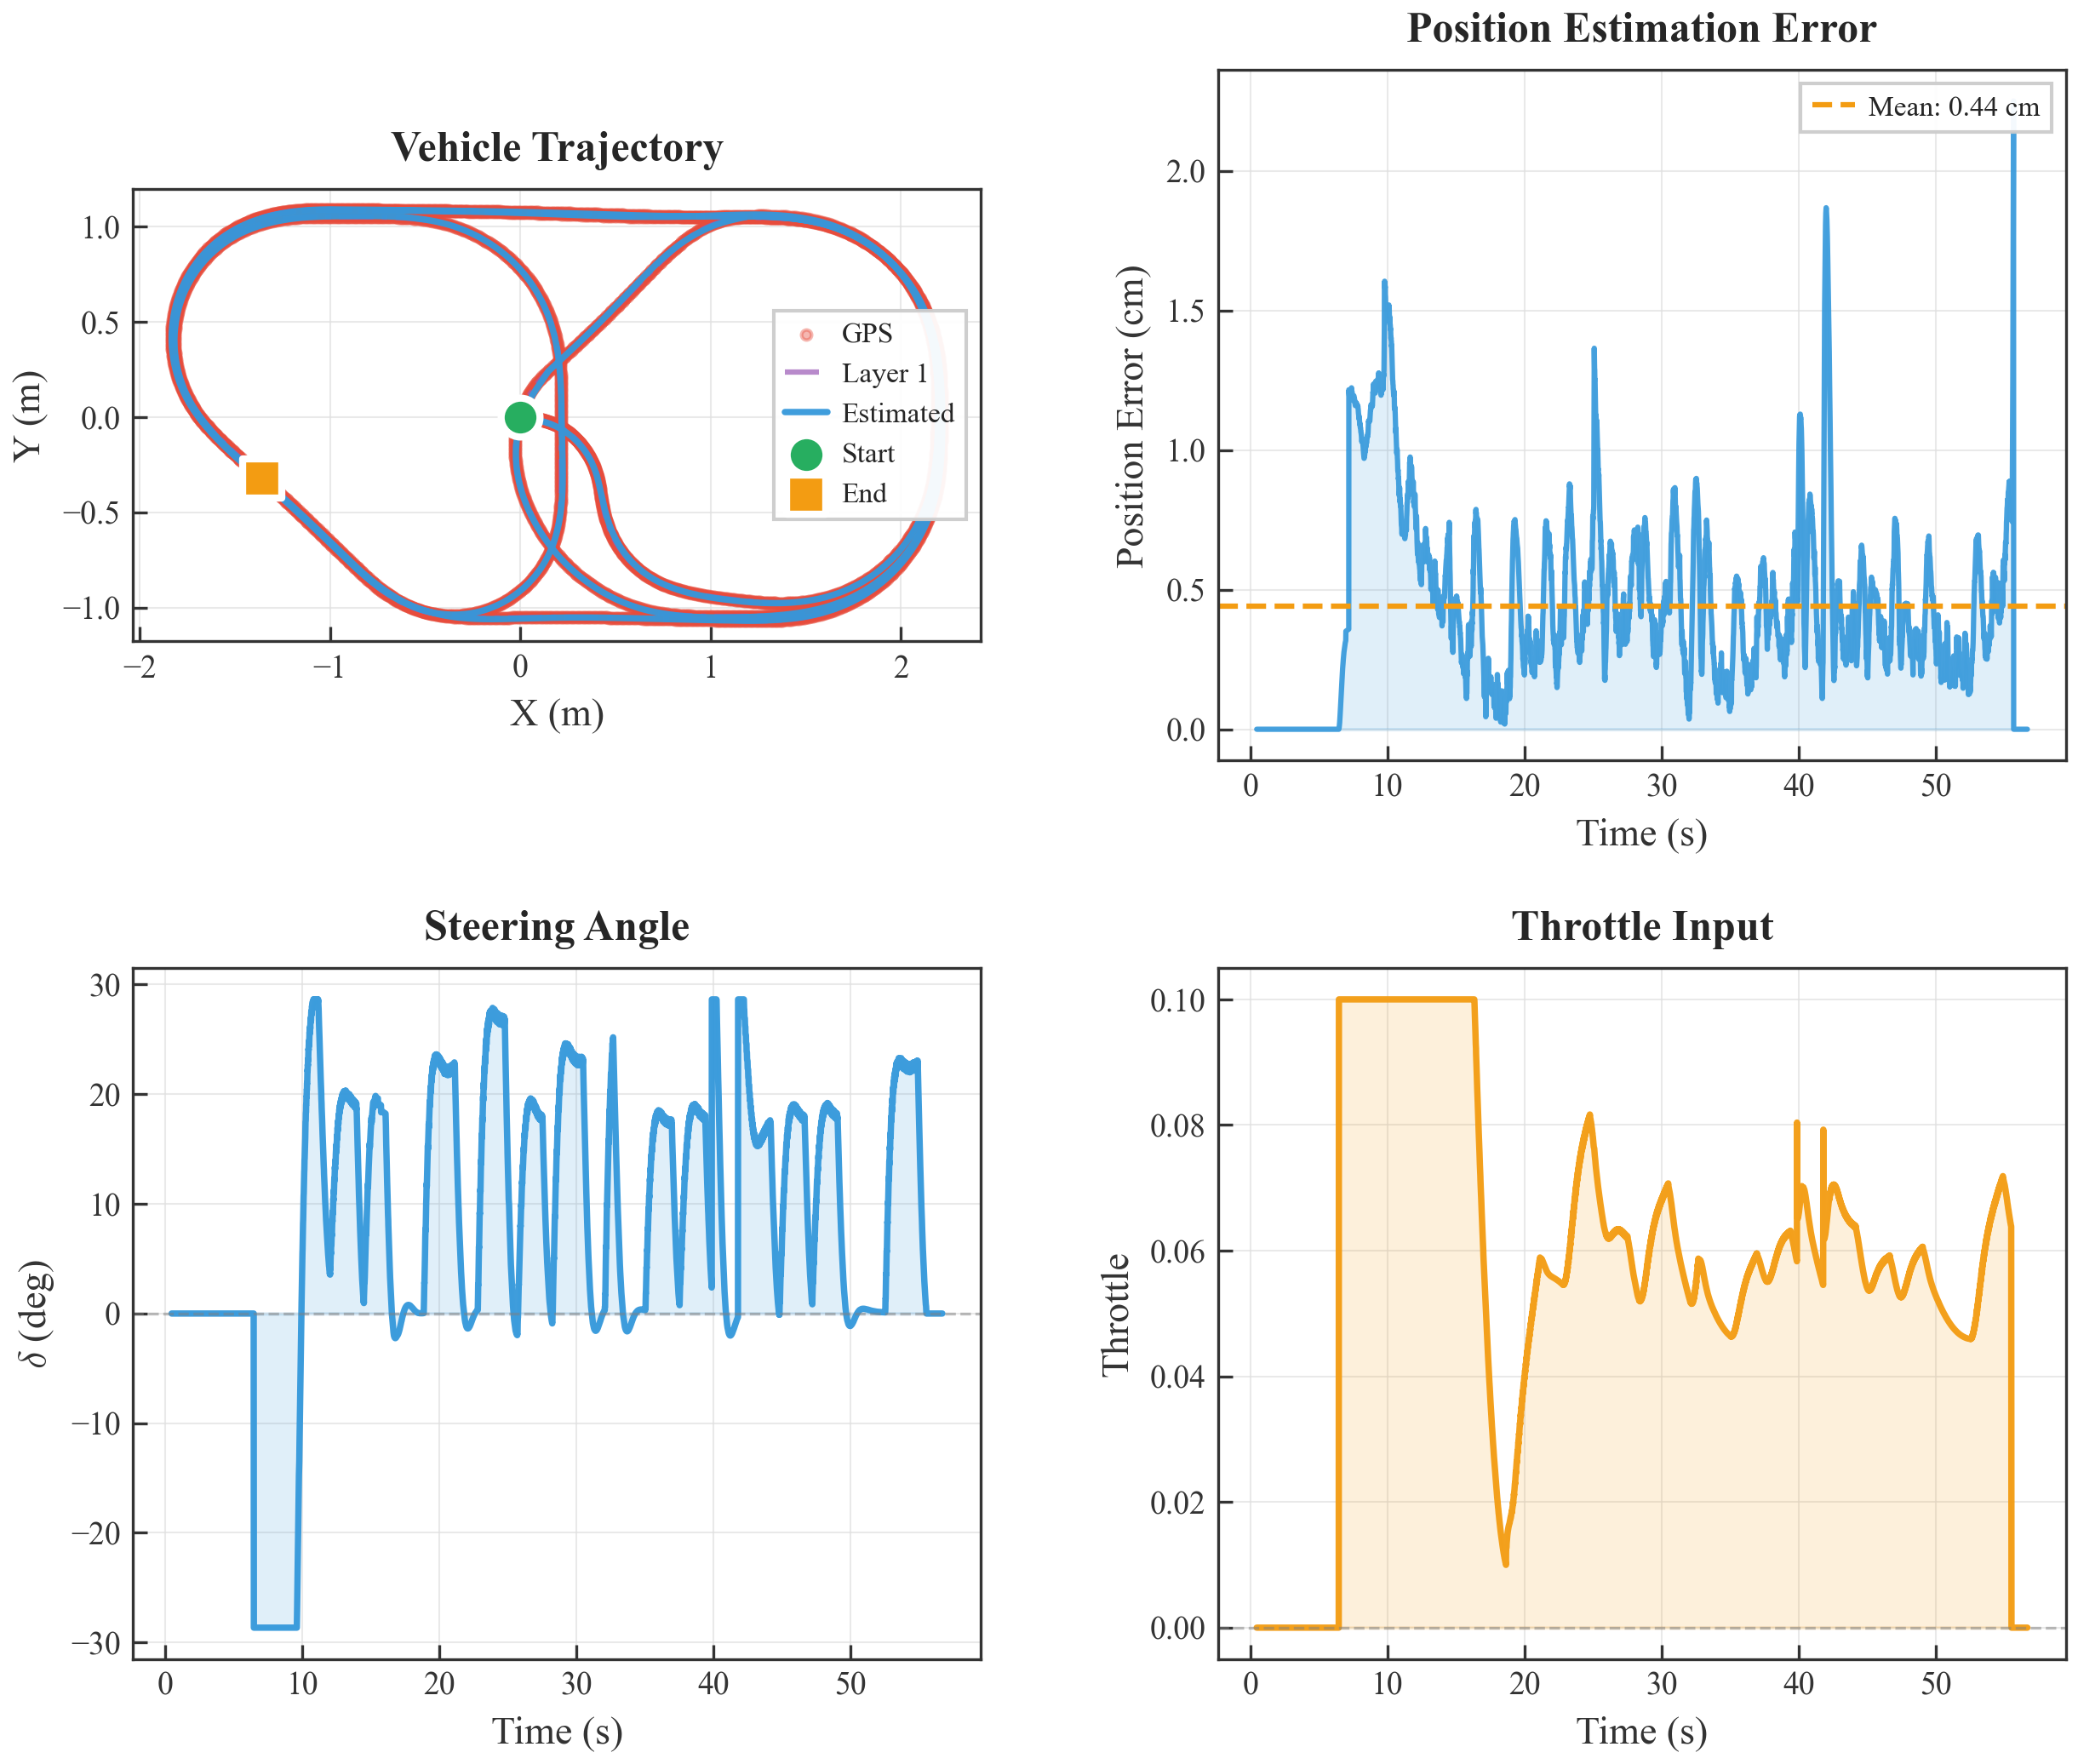
\includegraphics[width=0.7\linewidth]{traj_control_py.png}
    \caption{Vehicle trajectory, tracking error, and control inputs.}
    \label{fig:Trajectories_ch4}
\end{figure}

\subsubsection{State Estimation}
Figure~\ref{fig:state_estimate_wo} reports the state estimation results for both layers. The measured channels ($v_x$, $\psi$, and $r$) are recovered with high fidelity, while the unmeasured lateral velocity $v_y$ is also reconstructed through the coupling in the vehicle dynamics.

\begin{figure}[ht!]
    \centering
    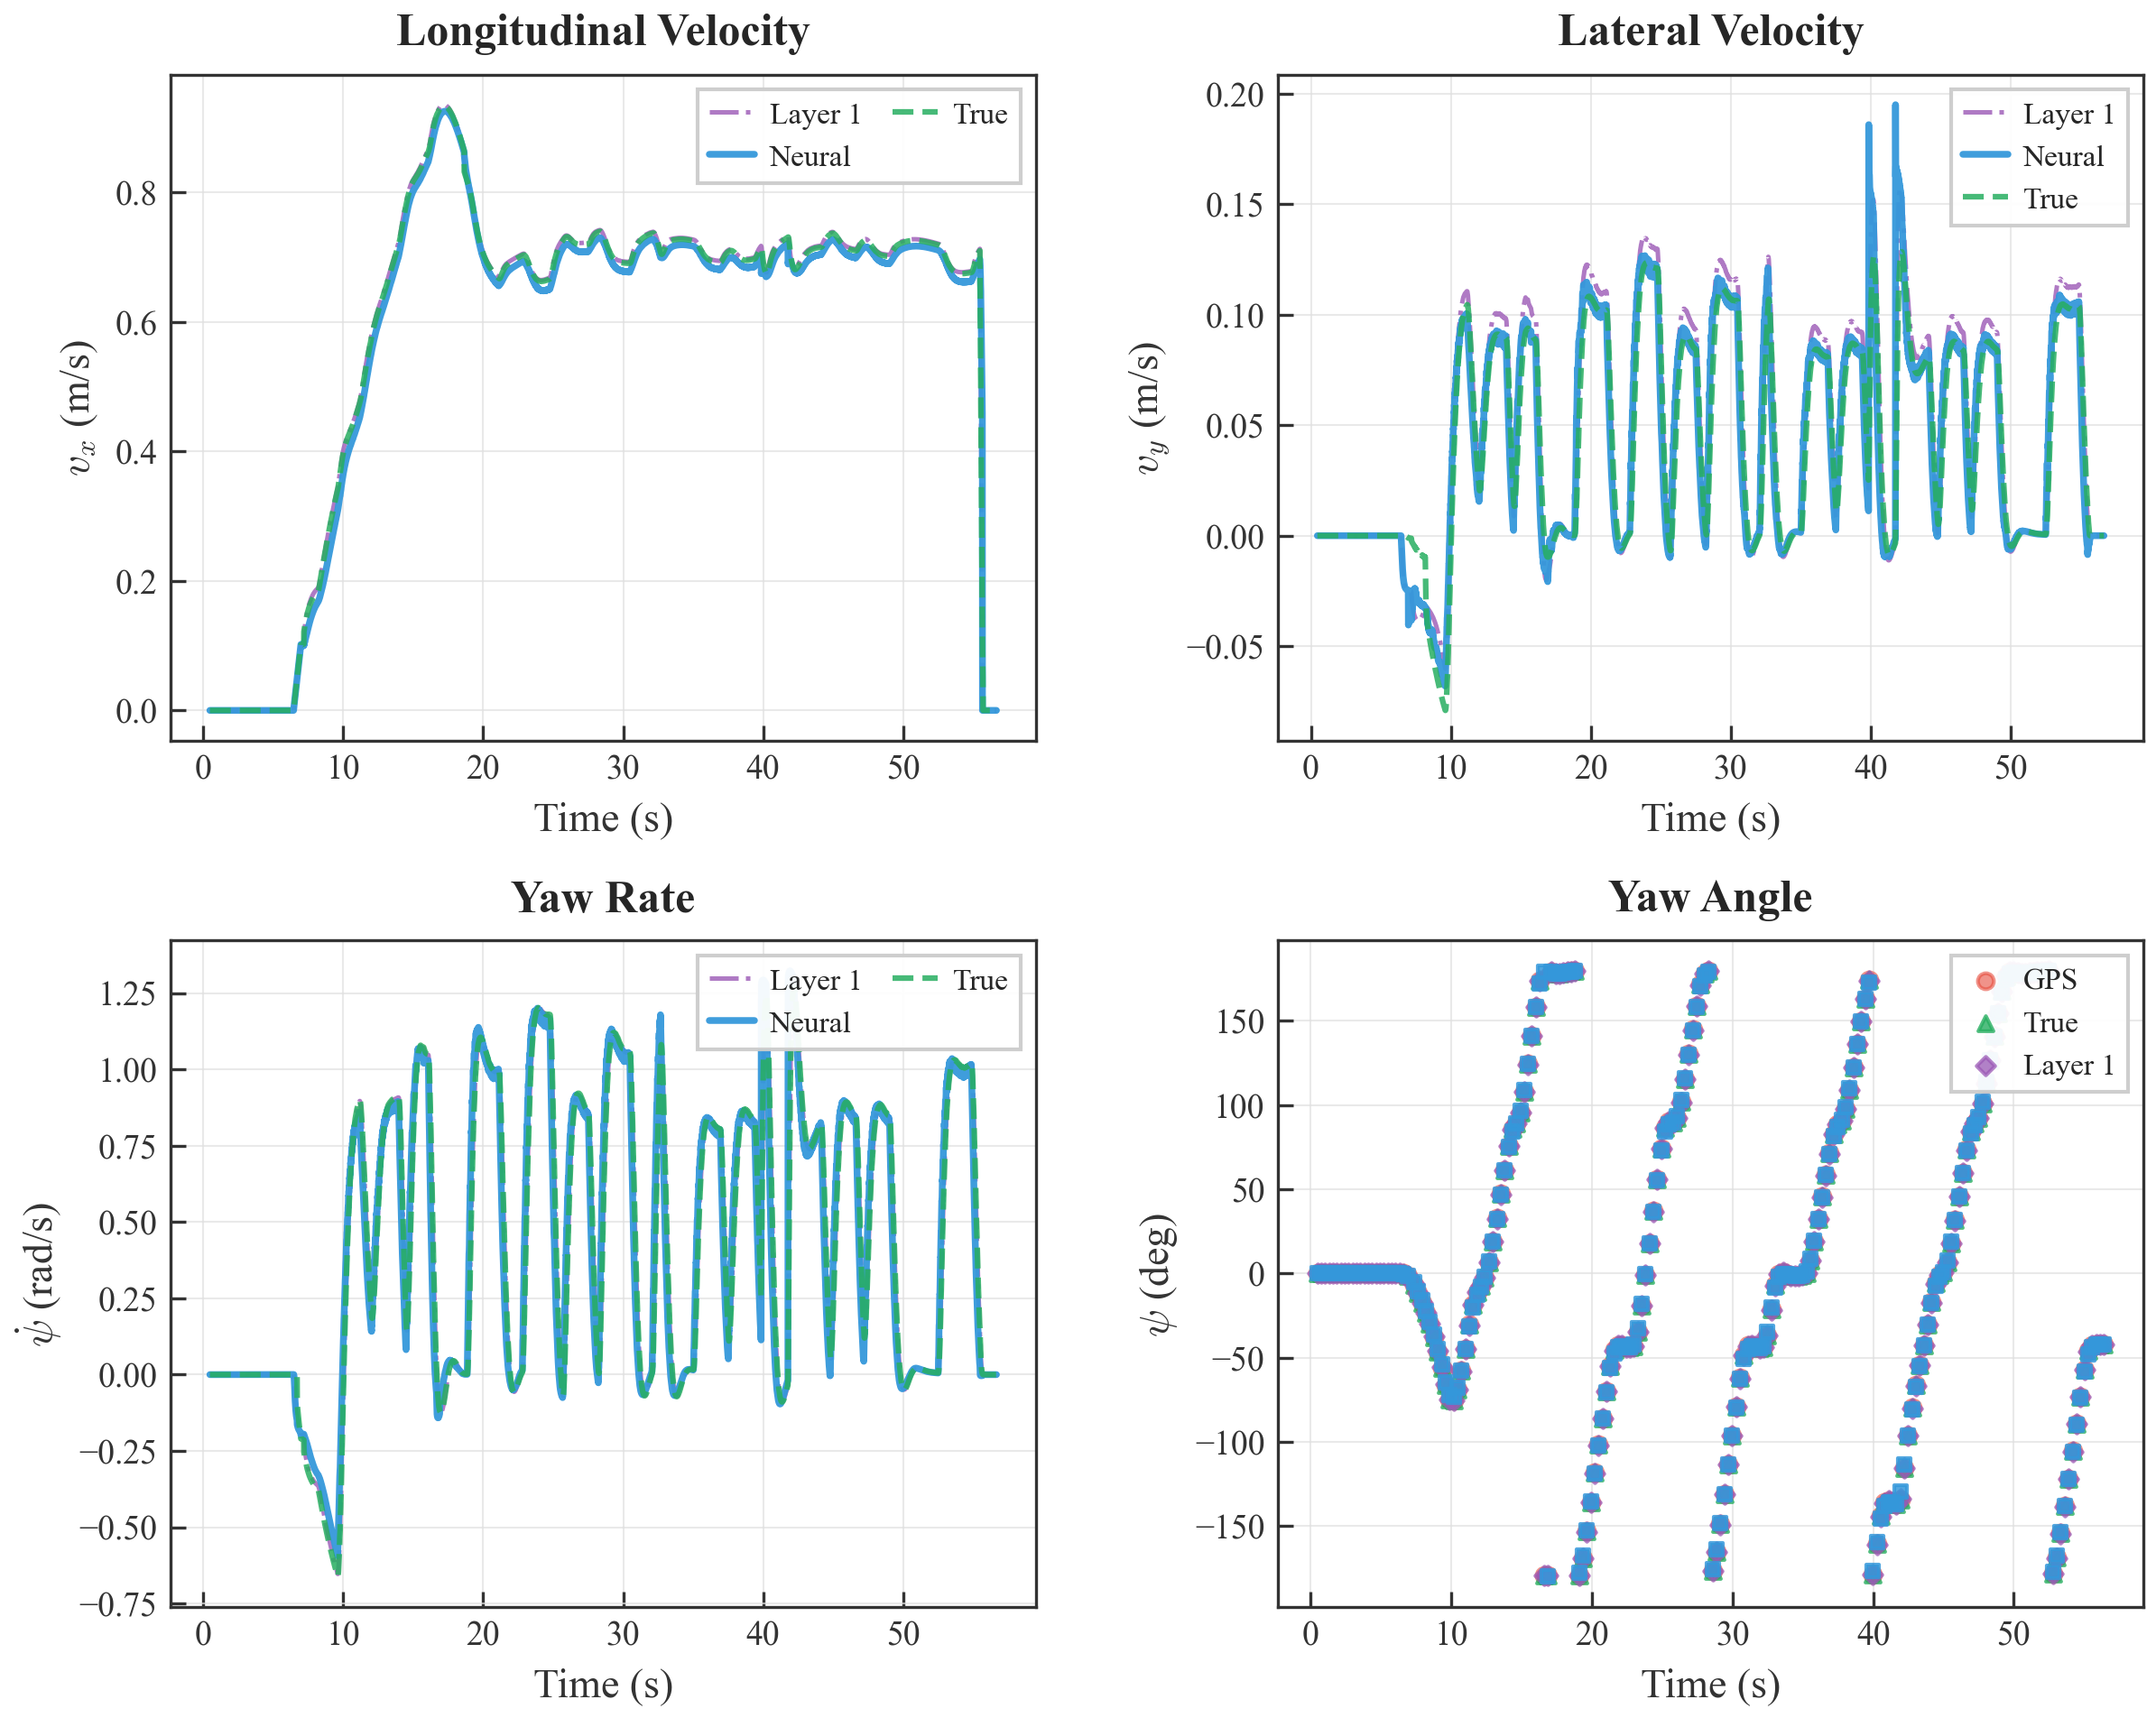
\includegraphics[width=0.7\linewidth]{State_est_py.png}
    \caption{Vehicle state-estimation results.}
    \label{fig:state_estimate_wo}
\end{figure}

\subsubsection{Tire-Force Residual Estimation}
Figure~\ref{fig:Uncertainty} presents the reconstruction of the unknown tire-force residuals $\mu_x = [f_{yf},\; f_{yr}]^\top$, comparing the estimates from Layer~1 (UIO) and Layer~2 (NAO). Both layers provide bounded estimates, while Layer~2 shows faster convergence and closer tracking of the true residual signals in this simulation. This improvement is attributed to the neural network's ability to learn the functional relationship $\mu_\theta(\hat{x})$, which refines the instantaneous UIO signal into a predictive model.

\begin{figure}[ht!]
    \centering
    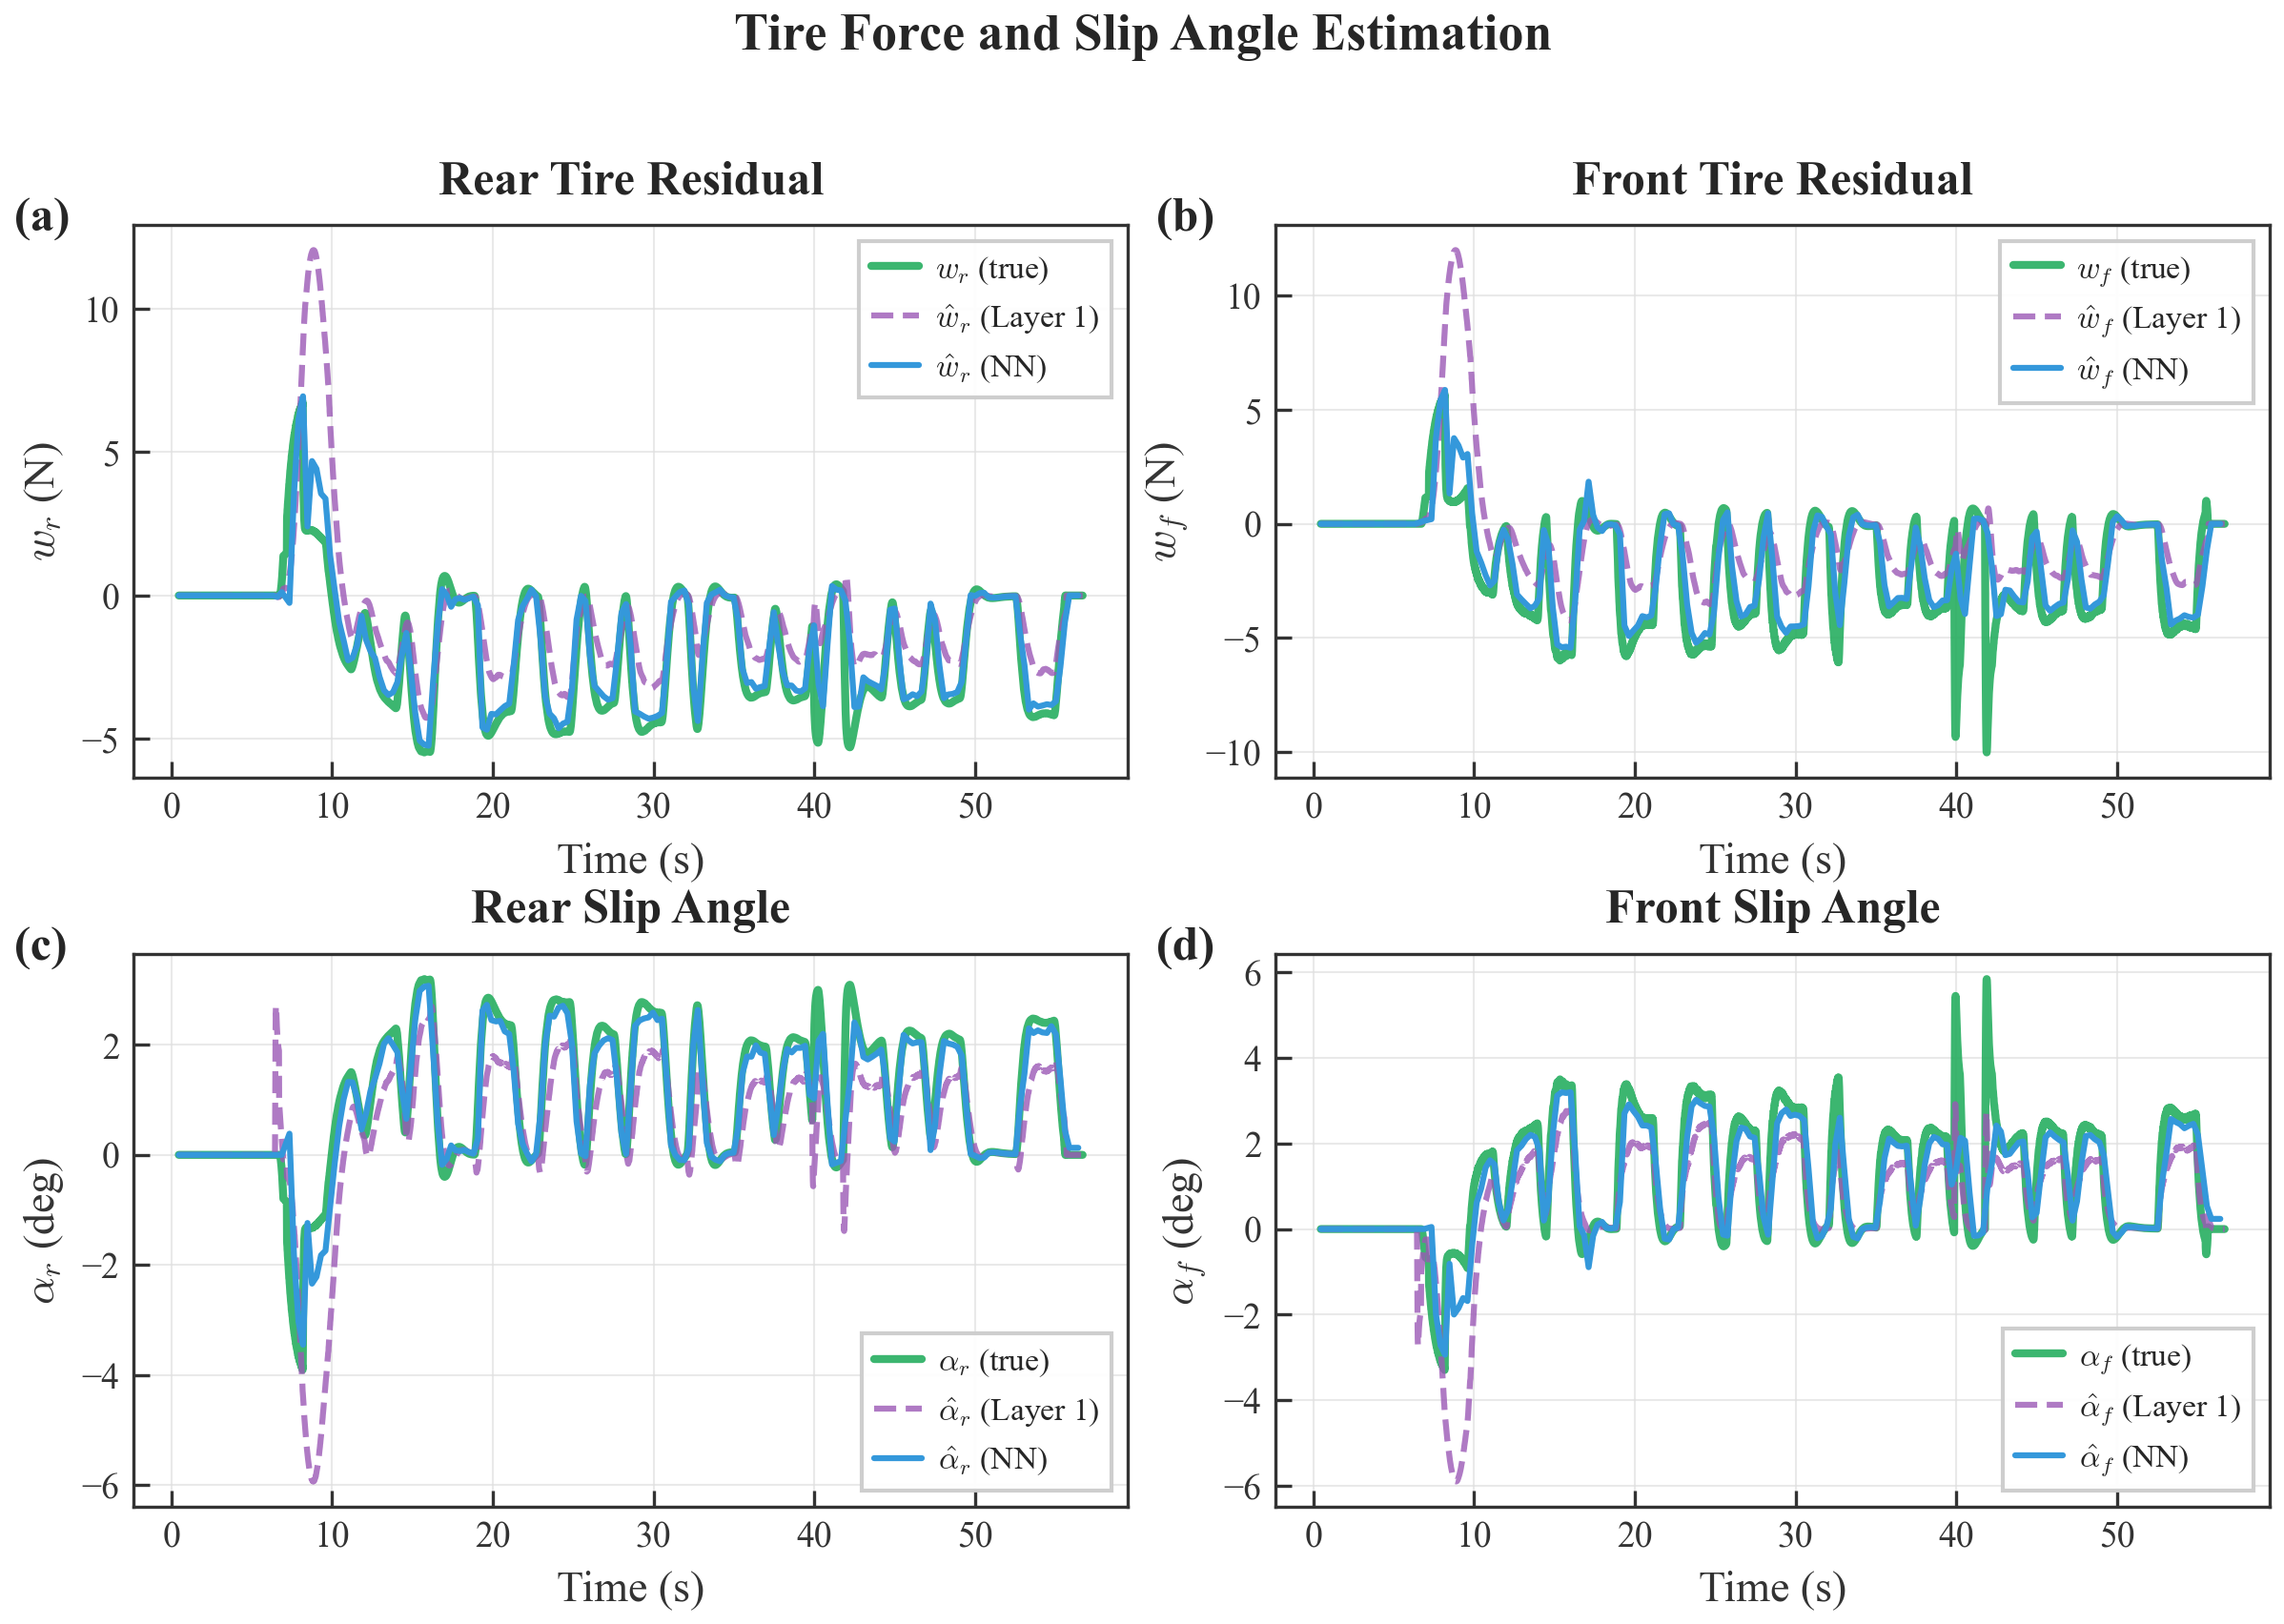
\includegraphics[width=0.7\linewidth]{tireforce_slip_py.png}
    \caption{Tire-force residual and slip-angle estimation.}
    \label{fig:Uncertainty}
\end{figure}

Overall, these results support the proposed two-layer hybrid design: the UIO (Layer~1) provides a stable physics-based supervisory signal with guaranteed bounded estimation, while the NAO (Layer~2) refines the reconstruction of the unknown tire-force residuals and improves the state estimates used for closed-loop trajectory tracking.



















%$$
% \textcolor{red}{***\text{ END ALI ***}}
%$$































\vspace*{-0.2cm}
%===============================
\section{Conclusion}\label{sec7}
\vspace*{-0.2cm}
%
This paper presented a hybrid estimation framework combining a regularized generalized UIO with neural online approximation of unmodeled dynamics. The UIO provides bounded physics-based estimates under LMI conditions, and these estimates supervise a neural observer whose error satisfies an $\mathcal L^2$ bound. The vehicle residual-learning result illustrates how tire-force reconstruction and learned residual correction can be separated in a teacher--student architecture. Future work will validate the approach on real driving data and develop a discrete-time embedded implementation.

\vspace*{-0.2cm}
%=================
% \bibliography{trust_ifac}
% \bibliographystyle{IEEEtran}
\bibliography{UIO_IFAC_refs}
%=================
\end{document}
